%\documentclass{article}
%\usepackage{pgfplots}
%\pgfplotsset{compat=1.7}
%
%\begin{document}
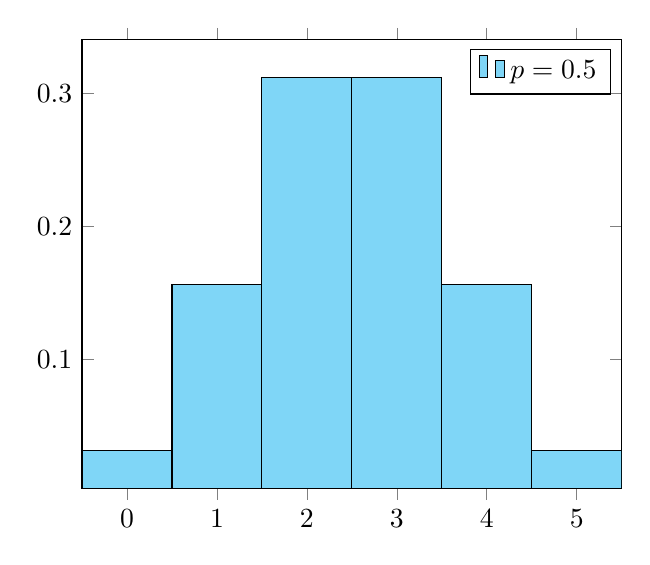
\begin{tikzpicture}[
    declare function={binom(\k,\n,\p)=\n!/(\k!*(\n-\k)!)*\p^\k*(1-\p)^(\n-\k);}
]
\begin{axis}[
    samples at={0,...,5},
    yticklabel style={
        /pgf/number format/fixed,
        /pgf/number format/fixed zerofill,
        /pgf/number format/precision=1
    },
    ybar=0pt, bar width=1
]
\addplot [fill=cyan, fill opacity=0.5] {binom(x,5,0.5)}; \addlegendentry{$p=0.5$}

\end{axis}
\end{tikzpicture}
%\end{document}